\documentclass[a4paper]{article}
\usepackage[margin=1in]{geometry}
\usepackage{polyglossia}
\setdefaultlanguage{danish}
\usepackage{graphicx}
\usepackage{float}
\usepackage[colorlinks,citecolor=blue,linkcolor=black,urlcolor=blue]{hyperref}
\usepackage{fancyref}
\setlength{\parindent}{0pt}

\title{E3SWE: Docker-compose services}
\author{Janus Bo Andersen  \\
	JA67494 \\
	Ingeniørhøjskolen i Aarhus, Campus Herning
	}

\date{\today}
\begin{document}

\maketitle

\section{Indledning}
Denne journal beskriver, hvordan en basal webservice sættes op vha. docker-compose.
Webservicen skal have en frontend/proxy-server (Nginx),
applikationslogik og applikationsserver (Flask) og en
databaseserver (PostgreSQL).
Den skal kunne tilgås på port 80 (standard Http).
Der skal tilknyttes et permanent lagermedium (Docker volume) til databasen.
\\\\
En tilsvarende webservice er sat op af forfatteren m.fl. ifm. E3PRO3, dog med Django i stedet for Flask \cite{team2}.

\section{Design}
Følgende figur illustrerer design af systemet.
Images er udvalgt fra officielle images på Docker Hub \cite{hub}.

\begin{figure}[H]
\centering
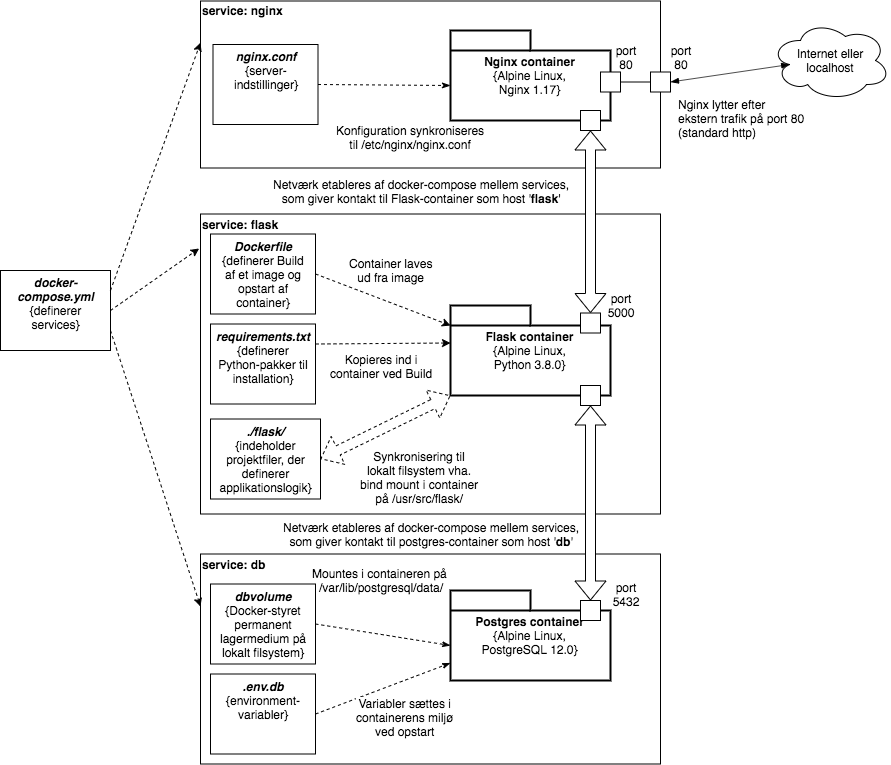
\includegraphics[width=14cm]{../img/flask-django.png}
\caption{Design og implementering (egen tilvirkning)\label{fig:design}}
\end{figure}

\section{Implementering}
Det er værd at bemærke princippet, at \textit{specifikke} versioner af images er valgt og fastlåst i implementering.
Implementerede versioner af images ses i figur~\ref{fig:design}.
I \texttt{docker-compose.yml}, er oprettelse af netværk (bridges) sat til at foretages automatisk af docker-compose,
der er derfor ikke navngivne netværksbroer. Alle containers kan forbindes via deres service/host-navne.
Al kode samt dette dokument kan ses på forfatterens Github \cite{janus}.
\texttt{Dockerfile} til Flask-app'en er gengivet her, fordi den er ``custom''.
\\\\
\begin{figure}[H]
\centering
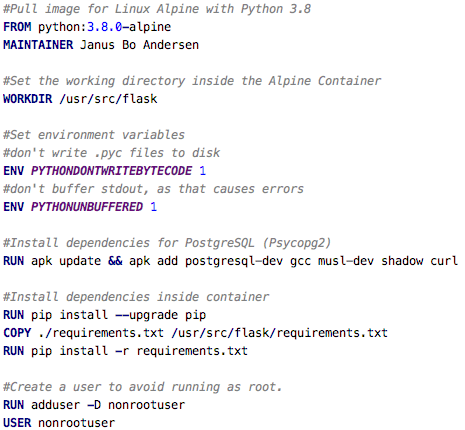
\includegraphics[width=12cm]{../img/dockerfile.png}
\caption{Dockerfile\label{fig:dockerfile}}
\end{figure}

\begin{par}
Systemet startes med \texttt{docker-compose up}.
Switch \texttt{-d} bruges for at køre services i baggrunden, og
\texttt{--build} for at tvinge et rebuild af alle containers.
\end{par}

\section{Test}
Koden er testet i Chrome på Mac med Docker Desktop ver. 2.1.0.4, Docker Engine ver. 19.03.4 og docker-compose 1.24.1.
Følgende figur viser viser OK testresultat for request på localhost:80.
\\\\
\begin{figure}[H]
\centering
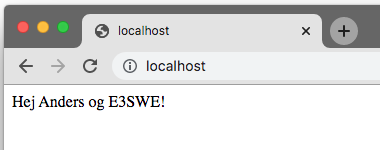
\includegraphics[width=7cm]{../img/test.png}
\caption{Testresultat: Browser\label{fig:test}}
\end{figure}

\begin{par}
Næste figur viser, at Nginx responderer på en Http-request, og proxyer til Flask.
\end{par}

\begin{figure}[H]
\centering
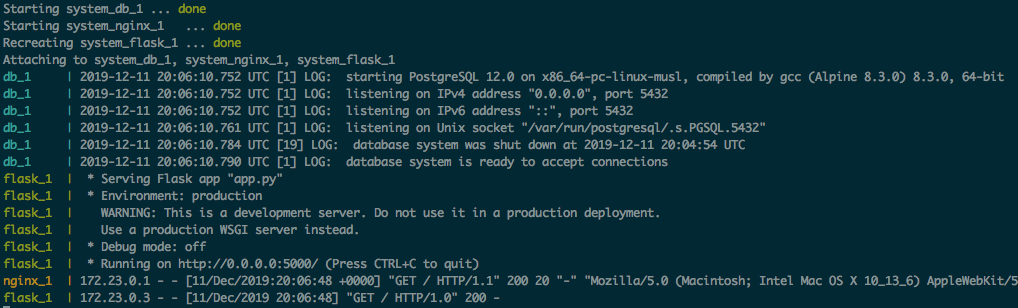
\includegraphics[width=16cm]{../img/test2.png}
\caption{Testresultat: Services\label{fig:test2}}
\end{figure}

\begin{par}
Systemet fungerer, som ønsket.
\end{par}

\section{Forbedringsmuligheder}
\begin{itemize}
	\item Flask's applikationsserver er ikke til produktion, og bør udskiftes med en WSGI-server med produktionskapacitet/sikkerhed, fx gunicorn.
	\item Databasen bliver ikke pt. benyttet af Flask. For at det kan virke godt, skal requirements.txt indeholde:
	\begin{itemize}
		\item psycopg2 (driver/adapter til PostgreSQL), og så bør postgresql-dev installeres via systemets package manager (APK).
		\item flask\_sqlalchemy (el.lign. toolkit/ORM til OOP).
		\item flask\_migrate (til at implementere schema-ændringer i databasen).
	\end{itemize}
	\item Opsætning, så der kan serves staticfiles.
	\item Opsætning af SSL/TLS-krypteret trafik (Https på port 443).
	\item Klargøring til deployment, fx til Heroku, AWS eller lignende.
	\item Noget \textit{langt mere} interessant indhold.
\end{itemize}

\section{Konklusion}
Denne journal har kort dokumenteret, hvordan en basal webservice sættes op.
Der er desuden givet et par forbedringsforslag til webservicen.
Al kode er tilgængelig på Github.

\begin{thebibliography}{9}
	\bibitem{team2} E3PRO3 Team 2, 2019. \emph{E3PRO3 Server setup},
	url: \url{https://github.com/AUTeam2/server-setup}.
	\bibitem{janus} Janus Bo Andersen. \emph{Github repo e3swe\_exam},
	url: \url{https://github.com/AUTeam2/server-setup}.
	\url{https://github.com/janusboandersen/e3swe_exam}.
	\bibitem{hub} Docker Hub. \emph{Official Docker Images},
	url: \url{https://hub.docker.com/search?type=image&image_filter=official}.
\end{thebibliography}

\end{document}